\documentclass[10pt]{article} 
\usepackage[letterpaper, portrait, margin=0.5in]{geometry} 
\usepackage{pbsi}

%\titleformat{\section}
  %{\normalfont\fontsize{20}{15}\bfseries}{\thesection}{1em}{}
%\titleformat{\subsection}
  %{\normalfont\fontsize{17}{0}\bfseries}{\thesection}{1em}{}
\usepackage{sectsty}
\sectionfont{\Huge}
\subsectionfont{\LARGE}

\usepackage{float}
\usepackage{graphicx}
\usepackage{subfig}


\usepackage{hyperref}
\hypersetup{colorlinks=true, linkcolor=blue, filecolor=magenta, urlcolor=cyan}

\usepackage{amsmath}

\begin{document} 
\title{\Huge \bsifamily Notes on OpenCL}
\author{\textit{by Ramkumar Narayanan}}
\date{}
\maketitle 
\tableofcontents
\newpage

% ----------------------------------------------------------------------------------------------------------------
{\color{red} \date{30-May-2020}}
\Large
\section{What is OpenCL?}
OpenCL is an industry standard for programming devices composed of a combination of CPU's, GPU's and other processors. This platform enables heterogeneous, distributed computing. OpenCL exposes the hardware. It does not attempt to hide it behind its abstractions. From a hardware perspective, we are tending towards obtaining maximum compute power per watt expenditure. 

Parallel hardware needs parallel software. This can be introduced with the concept of concurrency. Concurrency means running more than one stream of operations. Challenge is to find points of concurrency in a software system and express it as a source code. The resulting concurrent programs should deliver performance. Finding concurrency is pretty challengingand sometimes tricky. Coding up concurrency is the crus of the problem. Abstraction is often required to make the prallel program more manageable. 

\section{Programming Models}
This is a very high level description of the heteregeneous system. Basically there are two broad types of parallelism 1) \textit{\textbf{task parallelism}} and \textit{\textbf{data parallelism}}. Programmers break the problem down to individual tasks and then focus on how to bring about concurrency. This is easiest when tasks are independent. However, even when data is shared, this can be achieved. Concepts like load balancing comes here.

\begin{figure}[H]
  \centering
  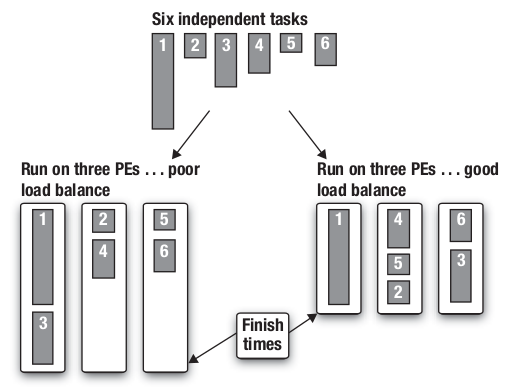
\includegraphics[scale=0.5]{./images/load_balancing.png}
  \caption{Load balancing of different tasks}
  \label{load balancing}
\end{figure}

In \textit{\textbf{data parallelism}} programmers update chunks of data elements in parallel. programmers think of their problems in terms of data elements.

\begin{figure}[H]
  \centering
  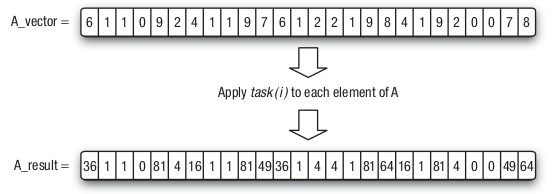
\includegraphics[scale=0.7]{./images/data_parallelism.png}
  \caption{Data parallelism where a single task is applied concurrently to many data elements}
  \label{data parallelism}
\end{figure}

\subsection{Platform Model}
\begin{enumerate}
	\item \textbf{\textit{Host:}} A device that controls all the OpenCL compatible devices. This is where the main entry point of the program. The host itself could be an OpenCL compatible device.
	\item \textbf{\textit{Compute Devices:}} Each graphics card or the CPU or FPGA's form what is called the compute device. All the compute devies are visible by the host.
	\item \textbf{\textit{Compute Units}} Like the several cores of the processor whether it be a GPU or a CPU. 
	\item \textbf{\textit{Processing Elements:}} Each core will have several small units that does the actual processing call the processing elements.
\end{enumerate}

\begin{figure}[H]
  \centering
  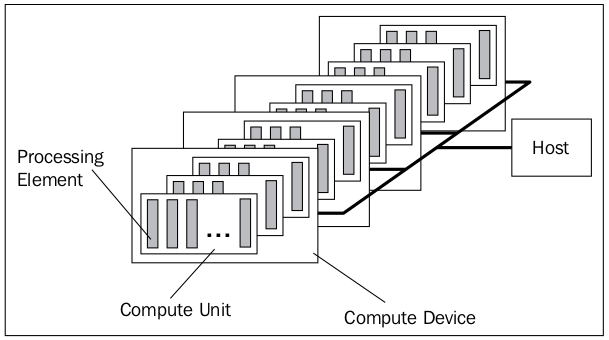
\includegraphics[scale=0.4]{./images/platform_model.png}
  \caption{OpenCL platform model}
  \label{platform_model}
\end{figure}

\subsection{Execution Model}
An OpenCL program has two distinct parts: 1) \textbf{\textit{Host}} program and 2) a collection of one or more \textbf{\textit{kernels}}. Host program runs on the host. Host program is our normal cpp or python code. OpenCL does not define how that is programmed - only how it interacts with the compute device(s).
\begin{enumerate}
	\item \textbf{\textit{OpenCL Kernels:}} Written in C language and compiled with the OpenCL C compiler.
	\item \textbf{\textit{Native Kernels:}} These functions are created outside OpenCL and accesssed within OpenCL through a function pointer.
\end{enumerate}

\textit{\textbf{How does a kernel execute on the OpenCL device?}} A kernel is defined on the host. The host program issues a command that submits the kernel for execution. When this command is issued, OpenCL runtime creates what is called the \textit{\textbf{index space}}. An instance of kernel executes for each point in the index space. Each instance of the executing kernel is called a \textit{\textbf{work item}}. A work item is identified by the coordinates in the index space. The behaviour of each kernel execution can differ due to branch statements in the execution. Work items are organized into work groups providing a more coarse grained decomposition of the index space. Work groups exactly span the index space. Work groups are of the same size. There are relative and global ID's for work groups and work items. Work items within a workgroup executes concurrently and workgroups may/may-not execute concurrently. The index space spans N-dimensions hence called the NDRange. Currently N can span 1, 2 or 3 dimensions. Let us take a look at the schemes using a 2D Range example.

\vspace{1cm}

\textit{\textbf{Notations:}}
\begin{enumerate}
	\item $G_x$ and $G_y$ - indicates the sizes of the index space.
	\item $W_x$ and $W_y$ - index space is chopped into so many work groups.
	\item $L_x$ and $L_y$ - individual work group size after chopping.
	\item $(g_x,g_y)$ - represents the global coordinates of the work item.
	\item $(w_x, w_y)$ - represents the coordinates of the work group.
	\item $(l_x,l_y)$ - represents work item coordinate within the work group.
\end{enumerate}

Take a look at the next image.

\begin{figure}[H]
  \centering
  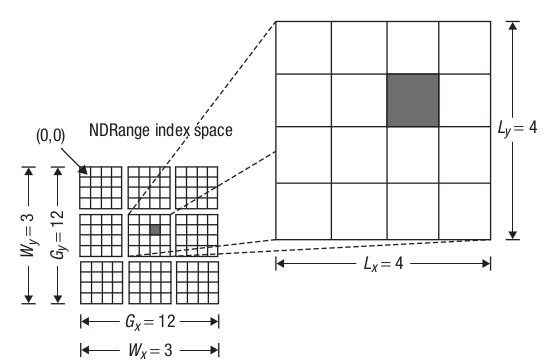
\includegraphics[scale=0.6]{./images/NDRange.png}
  \caption{NDrange, work group, work id}
  \label{}
\end{figure}

Number of work groups, $W_x=G_x/L_x$ and $W_y=G_y/L_y$.

\begin{enumerate}
	\item $(G_x,G_y)$ = $(12,12)$
	\item $(W_x,W_y)$ = $(3,3)$
	\item $(L_x,L_y)$ = $(4,4)$
	\item $(g_x,g_y)$ = $(6,5)$
	\item $(w_x,w_y)$ = $(1,1)$
	\item $(l_x,l_y)$ = $(2,1)$
\end{enumerate}

\subsubsection{Context:}
Computation of the kernels is always done on the OpenCL devices. However, the host has a very important job of setting up various stuff. For instance, the host defines the NDRange and the queues that control the details of how and when the kernels execute. All these definitions are contained in the API's within the OpenCL definition.

A context defines these environmental parameters within which the kernels are defined and executed. To be more precise, context is defined in the following terms,

\begin{enumerate}
	\item \textit{\textbf{Devices:}} A collection of OpenCL devices used by the host.
	\item \textit{\textbf{Kernels:}} A collection of OpenCL functions that run on the devices.
	\item \textit{\textbf{Program Objects:}} The source code and executables that implement kernels.
	\item \textit{\textbf{Memory Objects:}} a set of objects in memory that are visible to OpenCL devices and contain values that can be operated by instances of kernels.
\end{enumerate}



\end{document} 
 
